\section{Arkitektur}

Systemet er designet som en lagdelt 3-tier arkitektur, bestående af et \textbf{Presentation layer},
et \textbf{Application layer}, og et \textbf{Data layer}.
Arkitekturen følger en klassisk client-server model, hvor klienten (frontend) kommunikerer
med serveren via et API-lag.

\subsection{Arkitekturvalg og begrundelse}

Den lagdelte struktur er valgt med henblik på at sikre separation of concerns, høj vedligeholdbarhed og modularitet.
Ved at adskille præsentationslogik, forretningslogik og datalagring reduceres koblingen mellem systemets
komponenter, hvilket gør det muligt at ændre eller udvide ét lag uden at påvirke de øvrige lag i væsentlig grad.

Systemet er implementeret som en monolitisk applikation, da systemets kompleksitet ikke kræver microservices, og
det reducerer både udviklings- og deployment-kompleksitet.

Til API-laget er GraphQL valgt frem for en traditionel REST-arkitektur.
GraphQL giver klienten mulighed for at specificere præcist, hvilke data der ønskes
hvilket øger fleksibilitet og reducerer over-fetching af data og unødvendig netværks-trafik.
Dette bidrager til en øget performance og fleksibilitet i frontend-udviklingen\ (\cite{graphql}).

Til autentifikation anvendes en \texttt{REST}-baseret tilgang frem for \texttt{GraphQL}.
Login-processen er en simpel og veldefineret operation, som egner sig godt til en traditionel \texttt{POST}-request.
Ved at adskille autentifikationen fra \texttt{GraphQL}-endpointet, opnås en tydelig separation of concerns, hvor sikkerhed
og adgangskontrol kan håndteres isoleret.

Derudover gør en \texttt{REST}-baseret login-løsning det lettere at implementere sikkerhedsforanstaltninger som rate limiting
og beskyttelse mod brute force-angreb.
\texttt{GraphQL} anvendes således til fleksibel datahåndtering, mens \texttt{REST} benyttes til autentifikation, hvor en mere
simpel og kontrolleret arkitektur er fordelagtig.

Der implementeres også rate limiting på \texttt{GraphQL}-endpointet for at beskytte systemet mod overbelastning og misbrug.
Selvom autentifikation håndteres via \texttt{REST}, kan \texttt{GraphQL}-forespørgsler være komplekse og ressourcekrævende,
hvilket gør det nødvendigt at begrænse antallet af forespørgsler pr. tidsenhed for hver klient.
Dette sikrer både systemets stabilitet og fair ressourcefordeling mellem brugere.

\subsection{Presentation Layer}
Præsentationslaget er implementeret i Next.js og udgør brugerens interface med systemet.
Laget håndterer brugerinteraktioner, formularinput og præsentation af data, som hentes fra GraphQL API-et.

Server-side rendering (SSR) anvendes på udvalgte sider, for at optimere indlæsningstider
og forbedre brugeroplevelsen ved større datamængder.
State management håndteres primært via React's \textit{useState} samt context API\@.

Frontend-applikationen hostes via Vercel og er tilgængeligt på domænet \texttt{www.olros.online}.
Domæne-håndtering og DNS administreres via Cloudflare.

\subsection{Application Layer}

Applikationslaget består af en Node.js-server implementeret med Express og GraphQL.
GraphQL fungerer som API-lag, hvor resolvers håndterer queries og mutationer
og kommunikerer med service-laget, der implementerer forretnings-logikken.

Den interne arkitektur i applikationen følger en opdeling mellem resolvers, services og dataadgang,
hvilket understøtter modularitet og testbarhed.
Middleware anvendes til håndtering af autentifikation, logging og centraliseret fejlbehandling.

Api'et eksponeres lokalt på port 3000 og gøres offentligt tilgængelig vha. cloudflare tunnels\ (\cite{cloudflare_tunnels}).
Denne løsning muliggør sikker eksponering af specifikke services uden at åbne hele serverens netværksporte.
I produktionsmiljøet accepteres udelukkende requests fra \texttt{www.olros.online}, mens udviklingsmiljøet
også tillader adgang fra \texttt{localhost}.
Adgang til API'et fra eksterne verktøjer kræver gyldig autentifikation via JWT. Dermed sikres, at selv hvis endpointet
tilgås uden for browseren, kan data kun tilgås ved korrekt autorisation.

\subsection{Data Layer}

Databasen består af en PostgreSQL-database, hvor datastrukturen er modelleret som vist på Figur~\ref{fig:ER-diagram}.
Databasen er normaliseret til tredje normalform (3NF) for at minimere redundans og sikre konsistens. Dette indebærer, at
alle \texttt{non-key-attributes} er direkte afhængige af deres respektive \texttt{PRIMARY KEYS} og at der ikke forekommer
uønskede transitive afhængigheder.

Relationer mellem entiteter er modelleret gennem anvendelse af \texttt{Join-tables}, hvilket sikrer korrekt håndtering af
\texttt{many-to-many} relationer uden redundans.
Attributter er placeret i tabeller hvor de funktionelt hører til,
hvilket understøtter en klar og entydig datastruktur.

Enkelte steder er der foretaget bevidst denormalisering.
Eksempelvis lagres vinderen af en kamp eksplicit i \texttt{Match}-tabellen, selvom denne værdi kan udledes af kampens resultat.
Dette er gjort af hensyn til performance og for at reducere kompleksiteten i forespørgsler.
Attributter som eksempelvis player\_nr er afhængige af den specifikke relation mellem spiller og turnering og er derfor
korrekt placeret i relationstabeller.

Dataintegritet opretholdes gennem anvendelse af \texttt{PRIMARY}- og \texttt{FOREIGN}-keys, unikke constraints, samt
\texttt{NOT NULL}-begrænsninger.
Databasen er isoleret fra klientadgang og kan udelukkende tilgås via applikationslaget.

PostgreSQL kører i en container på backend-serveren og tilgås via en dedikeret dataforbindelse fra API'et.

\subsection{Sikkerhed}

Der er implementeret flere sikkerhedsmæssige foranstaltninger for at beskytte brugerdata og forhindre uautoriseret adgang.

CORS-konfigurationen er i produktionen begrænset til kun at acceptere requests fra \texttt{www.olros.online}.
Api'et eksponeres via Cloudflare Tunnels, hvilket reducerer angrebsfladen ved kun at offentliggøre specifikke
services frem for hele serverens netværksporte.

Al kommunikation foregår over HTTPS for at forhindre aflytning og man-in-the-middle-angreb.
Autentifikation håndteres ved brug af JSON Web Tokens og brugeradgangskoder lagres udelukkende som salted hashes genereret med \textit{bcrypt}.

\subsection{Kvalitetsattributter}

Arkitekturen understøtter flere centrale kvalitetsattributter:

\textbf{Maintainability:}
Den lagdelte struktur reducerer kobling mellem komponenter og gør det muligt at modificere eller
udvikle enkelte lag uden omfattende ændringer i resten af systemet.

\textbf{Modularity:}
Opdelingen mellem resolvers, services og dataadgang fremmer en modulær kodebase.

\textbf{Security:}
Adskillelse af data- og applikationslag, begrænset CORS-konfiguration, samt brug af HTTPS og JWT bidrager
til øget sikkerhed.

\textbf{Performance:}
Server-side rendering og GraphQL's selektive datahentning reducerer unødvendig datatransmission.

\textbf{Scalability:}
Selvom systemet er monolitisk, muliggør den lagdelte struktur fremtidig opdeling i separate services, hvis belastningen øges.

\begin{figure}[h!]
    \centering
    \fbox{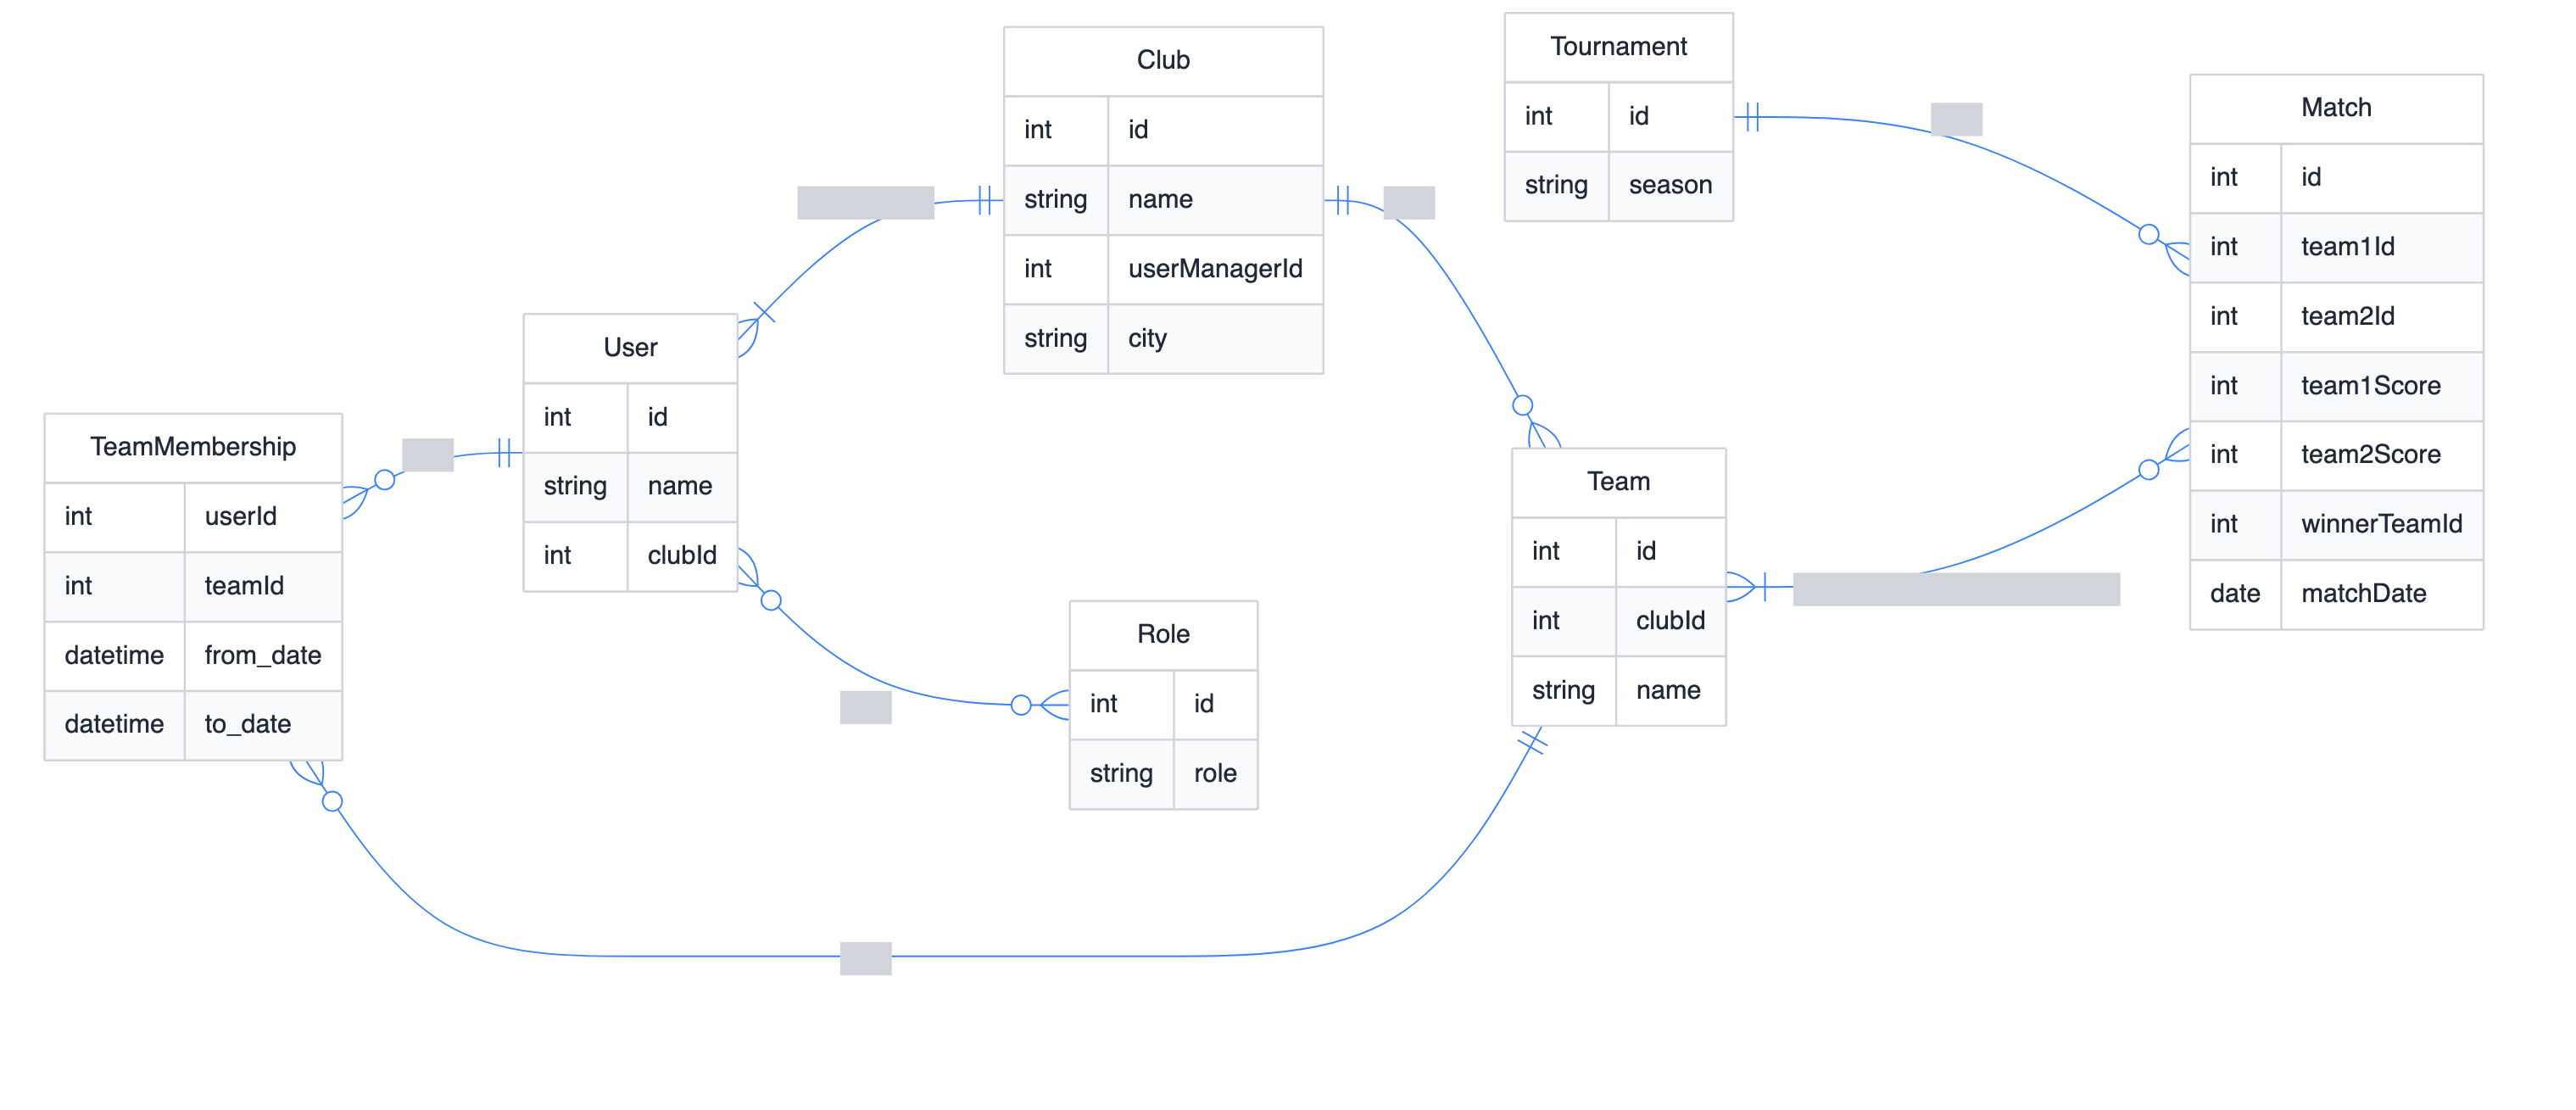
\includegraphics[width=1\textwidth]{Dokumenter/bilag/Diagrammer/ER-diagram}}
    \caption{ER-diagram}
    \label{fig:ER-diagram}
\end{figure}
